\documentclass[a4paper,oneside,12pt]{article}

\renewcommand{\small}{\fontsize{12}{12pt}\selectfont}
\renewcommand{\normalsize}{\fontsize{14}{14pt}\selectfont}
\renewcommand{\large}{\fontsize{16}{16pt}\selectfont}
\renewcommand{\baselinestretch}{1.5}

\usepackage[utf8x]{inputenc}
\usepackage{fontspec}
\setmainfont[Mapping=tex-text]{Times New Roman}

\usepackage[british,russian]{babel}
\usepackage[top=2cm,left=3cm,right=1cm,bottom=2cm]{geometry}
\usepackage{indentfirst}
\usepackage{hyperref}
\usepackage{underscore}
\usepackage{graphicx}
\RequirePackage{totcount}
\usepackage{float}
\usepackage{multirow}
\usepackage{ccaption}
	\captiondelim{ --- }
\usepackage{pdflscape}
\usepackage{array}
\usepackage{amsmath}
\regtotcounter{page}
\regtotcounter{figure}
\regtotcounter{table}
\newtotcounter{citnum}
\parindent=1.25cm
\def\oldbibitem{} 
	\let\oldbibitem=\bibitem
\def\bibitem{
	\stepcounter{citnum}\oldbibitem
}
\newcommand{\HRule}{\rule{4cm}{0.2mm}}
\makeatletter
\def\tableofcontents{\section*{\centering СОДЕРЖАНИЕ}\@starttoc{toc}}
\makeatother
\makeatletter
\renewcommand{\section}{\@startsection{section}{1}{1.25cm}{-\baselineskip}{0.5\baselineskip}{\normalfont\large\bfseries}}
\makeatother
\makeatletter
\renewcommand{\subsection}{\@startsection{subsection}{2}{1.25cm}{-\baselineskip}{0.5\baselineskip}{\normalfont\large\bfseries}}
\makeatother
\makeatletter
\renewcommand{\subsubsection}{\@startsection{subsubsection}{3}{1.25cm}{-\baselineskip}{0.5\baselineskip}{\normalfont\normalsize\bfseries}}
\makeatother
\makeatletter
\setlength\abovecaptionskip{2\p@}
\setlength\belowcaptionskip{1\p@}
\def\capfigure{figure}
\def\captable{table}
\long\def\@makecaption#1#2{%
  \vskip\abovecaptionskip
  \ifx\@captype\capfigure
      \centering #1~--~#2 \par
  \else
      \centering #1~--~#2 \par
  \fi
  \vskip\belowcaptionskip}
\renewcommand{\@biblabel}[1]{#1}
\makeatother
\usepackage{tabu}
\begin{document}
	\renewcommand{\figurename}{\small Рисунок}
	\renewcommand{\tablename}{\small Таблица}
	\thispagestyle{empty}
\begin{center}
Министерство образования и науки  Российской Федерации\\
Федеральное государственное автономное образовательное учреждение 
высшего профессионального образования\\
<<Уральский  федеральный университет\\ имени первого Президента России Б.Н.Ельцина>>\\
Физико-технологический институт\\
Кафедра вычислительной техники\\
\end{center}

\vspace{1cm}

\begin{flushright}
		\begin{minipage}{0.50\textwidth}
			\begin{flushleft}
				ДОПУСТИТЬ К ЗАЩИТЕ В ГЭК\\
				Зав. кафедрой \hrulefill\\
				\hrulefill \space \hrulefill\\
				{\small Ф. И. О.} \hspace{3cm} {\small (подпись)}\\
				<<\rule{1.5cm}{0.2mm}>> \hrulefill \space 201\rule{1cm}{0.2mm} г.\\
			\end{flushleft}
		\end{minipage}
\end{flushright}

\vspace{1cm}

\begin{center}
{\large Развитие синтаксического парсера русского языка}\\
\vspace{1cm}
Выпускная квалификационная работа магистра\\
Пояснительная записка\\
\vspace{3cm}
	\begin{tabular}{ l c l}
		Научный руководитель, доцент, к.т.н. & \HRule & А. Г. Кудрявцев\\
		Нормоконтролер, к.т.н. & \HRule & В. В. Ковалев\\
		Студент гр. Фт-47081 & \HRule & К. С. Лукинских\\		
	\end{tabular}\\
\vspace{3cm}
Екатеринбург\\
2013
\end{center}
\newpage
  \section*{\centering РЕФЕРАТ}

Пояснительная записка \total{page} страниц, \total{figure} рисунков, \total{table}
таблиц, \total{citnum} источников.

\emph{Актуальность работы}. С учётом тенденций к консолидации лингвистической 
информации и распространению технологий semantic web, наблюдается неспособность
имеющихся синтаксических парсеров русского языка к работе в меняющемся окружении. 
Следовательно, необходимо выделить наиболее эффективное решение из имеющихся
парсеров и модифицировать его, приспособив к работе с централизованными
хранилищами лингвистической информации.

\emph{Целью исследования} является развитие теоретического базиса технологии
взаимодействия синтаксических парсеров русского языка с централизованными
хранилищами лингвистической информации и разработка демонстрационного программного
продукта, эксплуатирующего данную технологию.

Для достижения поставленной цели необходимо решить следующие \emph{задачи}:
\begin{list}{\labelitemi}{\leftmargin=1.5cm}
  \item найти аналогичные синтаксические парсеры русского языка;
  \item выделить критерии сравнительного анализа аналогов;
  \item среди найденных парсеров"=аналогов определить парсер"=прототип,
  наиболее полно удовлетворяющий выделенным критериям;
  \item исследовать существующие технологии взаимодействия с онтологиями semantic
  web;
  \item разработать пакет моделей взаимодействия существующей системы с
  централизованными хранилищами лингвистической информации;
  \item разработать техническое задание на разработку модуля взаимодействия выбранного
  в качестве прототипа парсера с онтологиями semantic web;
  \item произвести проектирование описанного в техническом задании модуля;
  \item выполнить инженерную реализацию спроектированного модуля.
\end{list}

\emph{Объектом исследования} является синтаксический парсер русского языка.

\emph{Предметом исследования} являются технологии взаимодействия программных
средств с онтологиями semantic web.

\emph{Методы исследования}. Для разработки системы использовались методы
системотехники, проектирования информационных систем и технологии разработки
программного обеспечения.

\emph{Научная новизна работы}. Получен пакет моделей взаимодействия синтаксического
парсера русского языка с онтологиями semantic web.
\newpage
	\tableofcontents\newpage
  \section*{\centering{ОБОЗНАЧЕНИЯ И СОКРАЩЕНИЯ}}
\addcontentsline{toc}{section}{ОБОЗНАЧЕНИЯ И СОКРАЩЕНИЯ}
\begin{table}[H]
	\centering{
		\begin{tabular}{ p{3cm} p{12cm} }
			NLP & Natural language processing (обработка естественного языка)
		\end{tabular}
	}
\end{table}
\newpage
  \section*{\centering ВВЕДЕНИЕ}
\addcontentsline{toc}{section}{ВВЕДЕНИЕ}
Компьютерная лингвистика --- быстро развивающаяся область на стыке лингвистики, математики
и информатики. Достижения в этой области позволяют осуществлять обработку информации, представленной
в самой распространённой форме --- текстов на естественном языке. Такая обработка может осуществляться
автоматизированно, при минимальной поддержке со стороны человека, либо полностью автоматически, используя в качестве
источника данных обширнейшую коллекцию текстов в Интернете.

Работы по NLP ведутся с середины XX в. \cite{wiki_nlp}, и к настоящему времени разработана подробная методология
обработки касательно всех аспектов естественно-языковых данных (морфология, синтаксис, семантика и т.д.), реализовано
множество систем автоматической обработки естественного языка, в том числе парсеров. Существуют формализмы и языки программирования, 
изначально разрабатывавшиеся для решения проблемы обработки символьной информации.

Большинство проблемных ситуаций в автоматическом парсинге естественных языков вызвано несовершенством формальных грамматик, представляющих анализируемый язык внутри алгоритма обработки. Естественные языки плохо поддаются формализации, формальные грамматики неоднозначны и могут порождать на одном и том же высказывании множество различных результатов анализа, некоторые из которых будут полностью лишены смысла для человека.

В свою очередь, совершенствованию и уточнению существующих грамматик мешает отсутствие централизованных источников синтакических знаний, в результате чего каждый новый парсер должен иметь собственную базу правил используемой в алгоритме формальной грамматики. Помимо трудоёмкости формирования такой базы, значительно возрастает риск ошибки при наполнении базы, снижается полнота представленной в ней информации.

Концепция Semantic Web \cite{wiki_semantic_web}, с другой стороны, предлагает фреймворк, в рамках которого различные системы и приложения получают доступ к централизованным источникам знаний (например, в виде онтологий). Такой централизованный источник может обладать самой полной и корректной базой знаний об определённой предметной области (например, о синтаксисе конкретного естественного языка) и формироваться специалистами. Таким образом, использование внешних баз знаний при парсинге может существенно снизить неоднозначность, упростить разработку новых алгоритмов, сместив центр внимания на совершенствование используемого алгоритма, а не грамматики.

С этой точки зрения, наибольшей актуальностью подобная технология обладает именно в приложении к парсерам русского языка в связи с большей сложностью его формализации по сравнению с английским, для которого разработано и применяется множество различных методов парсинга.\newpage
  \indent \section{Проблематика развития синтаксического парсера русского языка}
В главе рассмотрены основные термины и понятия по теме работы, предложена технология поиска необходимой информации, произведен анализ аналогов, выбраны критерии для оценки аналогов и их оценка по выделенным критериям, выбран прототип, сформулированы цели и задачи диссертации.

\subsection{Основные термины и понятия}
Естественный язык --- язык племени, народа, нации, возникающий и развивающийся в данном этническом сообществе, в минимальной степени испытывающий сознательное воздействие, передающийся из поколения в поколение естественным путем \cite{academica_nl}.

Обработка естественного языка --- область компьютерных наук, искуственного интеллекта и лингвистики, изучающая взаимодействие между компьютерами и человеческими (естественными языками) \cite{wiki_nlp}.

Парсинг (синтаксический парсинг) --- процесс анализа строк символов на естественном или компьютерном языке в соответствии с правилами формальной грамматики \cite{wiki_parsing}.

Формальная грамматика --- множество правил продукции для строк формального языка, описывающих формирование строк из алфавита формального языка, соответствующих синтаксису этого языка \cite{wiki_fg}.

Локализация --- переработка существующего программного продукта с целью использования его в странах с другим языком \cite{academica_loc}.

Машинное обучение --- процесс, в результате которого машина (компьютер) способна показывать поведение, которое в неё не было явно заложено (запрограммировано) \cite{samuel}.

Semantic Web (семантическая паутина) --- инициатива World Wide Web Consortium по включению семантического содержимого в веб-страницы, структурированию современного веб-пространства на основе RDF \cite{wiki_semantic_web}.

Resource description framework (среда описания ресурса) --- это разработанная консорциумом Всемирной паутины модель для представления данных, в особенности --- метаданных, представляющая утверждения о ресурсах в виде, пригодном для машинной обработки \cite{wiki_rdf}. 

Онтология --- формальное представление знания в виде множества понятий и отношений между ними \cite{wiki_ont}.

\subsection{Литературно-аналитический обзор по теме работы}
Далее рассмотрена технология поиска информации по теме, предъявлены требования к аналогам, сформированы критерии их сравнения, описана технология выбора прототипа.

\subsubsection{Технология поиска информации}
Отбор аналогов осуществлялся в процессе поиска по следующим направлениям:
\begin{list}{\labelitemi}{\leftmargin=1.5cm}
	\item методы синтаксического парсинга (синтаксический парсинг, алгоритмы парсинга, формальные грамматики);
	\item методы синтаксического парсинга русского языка (сужение предыдущего направления применительно к русскому языку);
	\item синтаксические парсеры русского и английского языка (конкретные реализации, технические показатели и методы, лежащие в их основе).
\end{list}

Поиск производился преимущественно в сети Интернет с использованием алгоритма, представленного на рисунке \ref{fig:searchalg}

\begin{figure}[H]
	\centering
		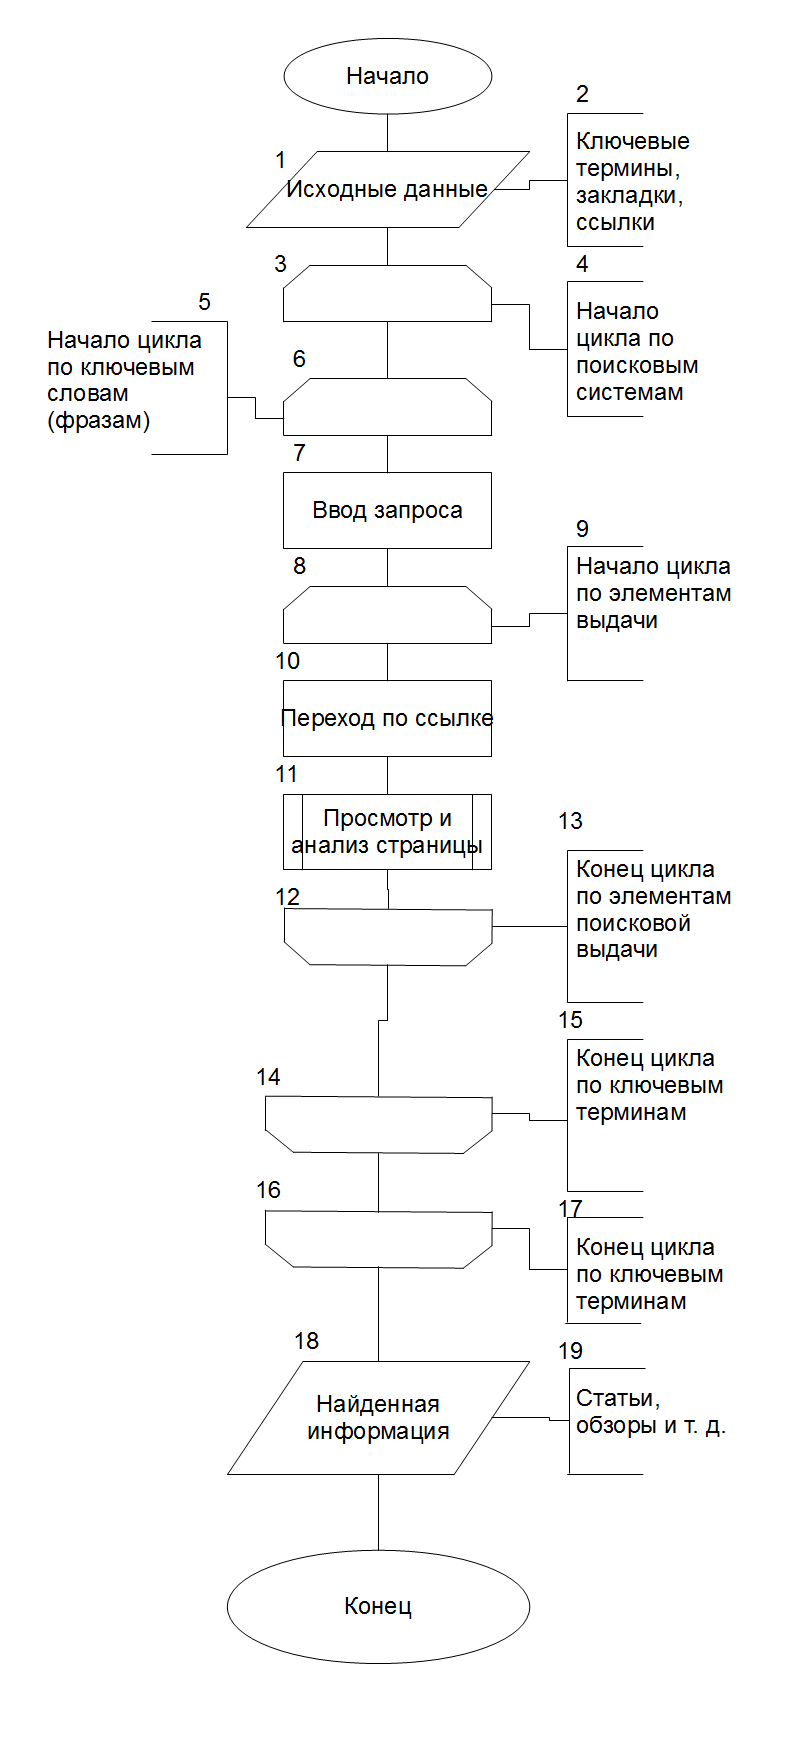
\includegraphics[scale=1.0]{images/searchalg.png}
	\caption{\small Алгоритм поиска информации в Интернете}
	\label{fig:searchalg}
\end{figure}

В приведённом на рисунке \ref{fig:searchalg} алгоритме использовались поисковые машины Google \cite{google}, Bing \cite{bing} и реже Yandex \cite{yandex}.

\subsubsection{Формирование требований к синтаксическому парсеру}
Выделение аналогов среди найденного производилось на основании максимального соответствия следующим предъявляемым к синтаксическим парсерам требованиям:
\begin{list}{\labelitemi}{\leftmargin=1.5cm}
	\item синтаксический парсер должен быть точным (минимальное число ошибок в результирующем дереве разбора, максимально корректное разрешение грамматически неоднозначных ситуаций) --- A;
	\item алгоритм синтаксического анализа должен быть эффективен (минимальная временная сложность алгоритма и сложность алгоритма по памяти, минимальное потребление памяти и процессорной мощности, максимальный потенциально возможный объём анализируемого текста) --- S;
	\item рассматриваемый аналог должен быть совместим с русским языком (минимальная степень специфичности грамматики по отношению к используемому языку, возможность реализовать формальную грамматику для русского языка на основе уже используемой парсером или наличие готовой) --- LS;
	\item входная информация должна быть в минимальной степени формализована (рассматриваемый аналог не должен требовать от входной информации предварительной обработки иными средствами естественноязыкового анализа) --- V.
\end{list}

\subsubsection{Критерии оценки аналогов}
Приведённые выше требования положены в основу четырёх критериев кортежной модели сравнения и оценки аналогов:\\
O = <A, S, LS, V; R>\\
где O --- интегральная оценка аналога, A --- критерий точности разбора, S --- критерий эффективности алгоритма, LS --- критерий простоты локализации грамматики, V --- критерий степени формализации входной информации, R --- матрица связи.

Методы оценки по выделенным критериям следующие:
\begin{list}{\labelitemi}{\leftmargin=1.5cm}
	\item A --- объективная нормированная процентная шкала, за нуль отсчёта взят минимальный показатель;
	\item S --- дискретная шкала, чем выше график производной функции сложности алгоритма, тем ниже оценка;
	\item LS --- дискретная шкала: 0.0 --- локализация грамматики невозможна, 0.25 --- для локализации необходима полная переработка грамматики, 0.50 --- достаточно изменить правила грамматики и провести машинное обучение, 0.75 --- достаточно отредактировать правила грамматики, 1.0 --- существует полноценная формальная грамматика русского языка;
	\item V --- дискретная шкала: 0.0 --- информация в виде метаданных, 0.50 --- информация в виде предварительно размеченного текста, 1.0 --- информация в виде необработанного текста.
\end{list}

Формула расчёта оценки аналога:

O \(= \alpha(A)*A + \alpha(S)*S + \alpha(LS)*LS + \alpha(V)*V\)\\
где 
\(\sum_{i=1}^{n} \alpha_i = 1\), \(\alpha_i\) --- весовой коэффициент соответствующего критерия, n --- количество критериев.

Найдём весовые коэффициенты методом попарного сравнения критериев Томаса Саати \cite{tsaati}. 
Будем использовать шкалу от 1 до 9, где: 
\begin{list}{\labelitemi}{\leftmargin=1.5cm}
  \item 1 --- равенство;
  \item 2 --- промежуточное значение;
  \item 3 --- слабое превосходство;
  \item 4 --- промежуточное значение;
  \item 5 --- сильное превосходство;
  \item 6 --- промежуточное значение;
  \item 7 --- значительное превосходство;
  \item 8 --- промежуточное значение;
  \item 9 --- абсолютное превосходство.
\end{list}
Матрица попарного сравнение представлена в таблице \ref{tab:crit}.

\begin{table}[H]
\centering
\caption{Матрица попарного сравнения критериев}
{\small 
\begin{tabu}to \textwidth{ | X[c] | X[c] | X[c] | X[c] | X[c] | X[c] | X[c] | }
	\hline
          & A   & S   & LS  & V & Среднее & Вес  \\ \hline
	A     & 1   & 3   & 4   & 7 & 3.75    & 0.51 \\
	S     & 1/3 & 1   & 3   & 5 & 2.33    & 0.31 \\
	LS    & 1/4 & 1/3 & 1   & 2 & 0.90    & 0.12 \\
	V     & 1/7 & 1/5 & 1/2 & 1 & 0.43    & 0.06 \\ \hline
	Сумма &     &     &     &   & 7.41    & 1.00 \\
	\hline
\end{tabu}
}
\label{tab:crit}
\end{table}

\subsubsection{Обзор найденных аналогов}

\subsubsection{Выбор прототипа}
Выделенные в требованиях характеристики для найденных аналогов были определены и сведены в таблице \ref{tab:obj}.

\begin{table}[H]
\centering
\caption{Результат объективной оценки аналогов по критериям}
{\small 
\begin{tabu}to \textwidth{ | X[c] | X[c] | X[c] | X[c] | X[c] | }
	\hline
    Аналог/Критерий & A    & S                & LS   & V   \\ \hline
	BLA                      & 75.9 & \(O(n^3)\)       & 0.50 & 1.0 \\ \hline
	SP                       & 72.8 & \(O(n^3*|G|^2)\) & 0.50 & 1.0 \\ \hline
	RG                       & 78.1 & \(O(n^5)\)       & 0.50 & 1.0 \\ \hline
	CYK                      & 66.6 & \(O(n^3*|G|)\)   & 0.75 & 0.5 \\ \hline
	IOA                      & 56.0 & \(O(n^3)\)       & 0.50 & 1.0 \\ \hline
	EA                       & 78.0 & \(O(n^3)\)       & 0.75 & 0.5 \\ \hline
	LGP                      & 73.0 & \(O(n^3)\)       & 1.00 & 1.0 \\ 
	\hline
\end{tabu}
}
\label{tab:obj}
\end{table}

С учётом приведённой ранее системы выставления оценок, объективные показатели были переведены в значения на соответствющих шкалах и нормированы. Результат представлен в таблице \ref{tab:scales}.

\begin{table}[H]
\centering
\caption{Результат нормированной оценки аналогов по шкалам критериев}
{\small 
\begin{tabu}to \textwidth{ | X[c] | X[c] | X[c] | X[c] | X[c] | }
	\hline
    Аналог/Критерий          & A    & S     & LS   & V   \\ \hline
	BLA                      & 0.97 & 1.00  & 0.50 & 1.0 \\ \hline
	SP                       & 0.93 & 0.50  & 0.50 & 1.0 \\ \hline
	RG                       & 1.00 & 0.00  & 0.50 & 1.0 \\ \hline
	CYK                      & 0.85 & 0.75  & 0.75 & 0.5 \\ \hline
	IOA                      & 0.72 & 1.00  & 0.50 & 1.0 \\ \hline
	EA                       & 1.00 & 1.00  & 0.75 & 0.5 \\ \hline
	LGP                      & 0.93 & 1.00  & 1.00 & 1.0 \\ 
	\hline
\end{tabu}
}
\label{tab:scales}
\end{table}

Взвешенные оценки, полученные умножением оценки по шкале на соответствующий весовой коэффициент, приведены в таблице \ref{tab:weight}.

\begin{table}[H]
\centering
\caption{Результат оценки аналогов по шкалам критериев}
{\small 
\begin{tabu}to \textwidth{ | X[c] | X[c] | X[c] | X[c] | X[c] | X[c] | }
	\hline
    Аналог/Крит.             & A    & S     & LS   & V    & Сумма \\ \hline
	BLA                      & 0.49 & 0.31  & 0.06 & 0.06 & 0.92  \\ \hline
	SP                       & 0.47 & 0.16  & 0.06 & 0.06 & 0.75  \\ \hline
	RG                       & 0.51 & 0.00  & 0.06 & 0.06 & 0.63  \\ \hline
	CYK                      & 0.43 & 0.23  & 0.09 & 0.03 & 0.78  \\ \hline
	IOA                      & 0.37 & 0.31  & 0.06 & 0.06 & 0.80  \\ \hline
	EA                       & 0.51 & 0.31  & 0.09 & 0.03 & 0.94  \\ \hline
	LGP                      & 0.47 & 0.31  & 0.12 & 0.06 & 0.96  \\ 
	\hline
\end{tabu}
}
\label{tab:weight}
\end{table}

\subsection{Критика прототипа}\newpage
  \renewcommand*{\refname}{}
\section*{\centering СПИСОК ИСПОЛЬЗОВАННЫХ ИСТОЧНИКОВ}
\addcontentsline{toc}{section}{СПИСОК ИСПОЛЬЗОВАННЫХ ИСТОЧНИКОВ}
\begin{thebibliography}{99}	
	\bibitem{academica_nl}
	Словарь социолингвистических терминов. Академика. [Электронный ресурс] --- Режим доступа: \url{http://sociolinguistics.academic.ru/185}. Дата обращения 21.05.2013.

	\bibitem{wiki_nlp}
	Natural language processing [Электронный ресурс] --- Режим доступа: \url{http://en.wikipedia.org/wiki/Natural_language_processing}. Дата обращения 20.05.2013.	

	\bibitem{wiki_parsing}
	Parsing [Электронный ресурс] --- Режим доступа: \url{http://en.wikipedia.org/wiki/Parsing}. Дата обращения 21.05.2013.	

	\bibitem{wiki_fg}
	Formal grammar [Электронный ресурс] --- Режим доступа: \url{https://en.wikipedia.org/wiki/Formal_grammar}. Дата обращения 21.05.2013.

	\bibitem{academica_loc}
	Финансовый словарь. Академика. [Электронный ресурс] --- Режим доступа: \url{http://dic.academic.ru/dic.nsf/fin_enc/24769}. Дата обращения 21.05.2013.

	\bibitem{samuel}
	Samuel A. L. Some Studies in Machine Learning Using the Game of Checkers. // IBM Journal. 1959.	

	\bibitem{wiki_semantic_web} 
	Semantic Web [Электронный ресурс] --- Режим доступа: \url{http://en.wikipedia.org/wiki/Semantic_Web}. Дата обращения 20.05.2013.	

	\bibitem{wiki_rdf}
	Resource description framework [Электронный ресурс] --- Режим доступа: \url{http://ru.wikipedia.org/wiki/Resource_Description_Framework}. Дата обращения 21.05.2013.	

	\bibitem{wiki_ont}
	Ontology [Электронный ресурс] --- Режим доступа: \url{http://en.wikipedia.org/wiki/Ontology_(information_science)}. Дата обращения 21.05.2013. 

	\bibitem{google}
	Google Search [Электронный ресурс] --- Режим доступа: \url{http://google.com}. Дата обращения 20.05.2013.

	\bibitem{bing}
	Microsoft Bing [Электронный ресурс] --- Режим доступа: \url{http://bing.com}. Дата обращения 20.05.2013.

	\bibitem{yandex}
	Yandex [Электронный ресурс] --- Режим доступа: \url{http://ya.ru}. Дата обращения 20.05.2013.

	\bibitem{tsaati}
	Саати, Т. Принятие решений. Метод анализа иерархий. Издательство: М.: Радио и связь. 1993.	

	\bibitem{eisner}
	Eisner J.M. Three New Probabilistic Models for Dependency Parsing: An Exploration. // Proceedings of the 16th International Conference on Computational Linguistics. – 1996.

	\bibitem{wiki_cyk}
	CYK algorithm [Электронный ресурс] --- Режим доступа: \url{http://en.wikipedia.org/wiki/CYK_algorithm}. Дата обращения 28.05.2013.	

	\bibitem{webbe}
	Webbe B. Chart Parsing: The Earley Algorithm. --- 2007.

	\bibitem{sleator}
	Sleator D.D.K. Parsing English with a Link Grammar. --- 1991.

	\bibitem{wiki_modelling}
	Моделирование [Электронный ресурс] --- Режим доступа: \url{http://ru.wikipedia.org/wiki/Моделирование}. Дата обращения 30.05.2013.

	\bibitem{uemov}
	Уёмов А. И. Логические основы метода моделирования, М.: Мысль, 1971.

	\bibitem{gold}
	Гольдштейн С.Л., Ткаченко Т.Я. Введение в системологию и системотехнику.

	\bibitem{abiparser}
	Link Grammar Parser [Электронный ресурс] --- Режим доступа: \url{http://www.abisource.com/projects/link-grammar/}. Дата обращения: 03.06.2013.	

	\bibitem{api}
	The Link Parser API [Электронный ресурс] --- Режим доступа: \url{http://www.abisource.com/projects/link-grammar/api/index.html}. Дата обращения 03.06.2013.	

	\bibitem{gpl}
	Стандартная общественная лицензия GNU [Электронный ресурс] --- Режим доступа: \url{http://www.gnu.org/licenses/gpl.html}. Дата обращения: 03.06.2013.

	\bibitem{haskell}
	The Haskell Programming Language [Электронный ресурс] --- Режим доступа: \url{http://www.haskell.org/haskellwiki/Haskell}. Дата обращения: 03.06.2013.

	\bibitem{haskell2010}
	Announcing Haskell 2010 [Электронный ресурс] --- Режим доступа: \url{http://www.haskell.org/pipermail/haskell/2009-November/021750.html}. Дата обращения: 04.06.2013.
\end{thebibliography}\newpage
\end{document}
